\documentclass[1p]{elsarticle}
\usepackage{graphicx}
\usepackage{caption}
\usepackage{amsmath}
\usepackage{hyperref}
\usepackage{float}

\journal{Building and Environment}

\title{Supplementary Material for \\ Physics-Informed Neural Networks for Robust Thermal Comfort Prediction: Overcoming Data Quality Limitations Through Physiological Constraints}
% \author{[Your Name]}
\date{}

\begin{document}

\maketitle

\section*{Table S1. $TSV$ value datatype breakdown}
\begin{table}[htbp]
    \centering
    \begin{tabular}{|c|c|c|c|c|}
    \hline
    Source & Float (\%) & Integer (\%) & Float (\#) & Integer (\#) \\
    \hline
    ASHRAE & 9.05 & 90.95 & 9866 & 99167 \\\hline
    China & 10.53 & 89.47 & 4421 & 37557 \\\hline
    Global & 9.46 & 90.54 & 14287 & 136724 \\\hline
    \end{tabular}
    % \caption{Breakdown of integer and float}
    \label{tab:int-float}
\end{table}

\section*{Table S2. Database alignment mapping between ASHRAE II and Chinese Thermal Comfort Databases}
\begin{table}[h!]
  \centering
  \resizebox{\textwidth}{!}{%
    \begin{tabular}{|l|l|l|l|}
      \hline
      \textbf{Unified New Name} & \textbf{Chinese (Set 1) Column} & \textbf{ASHRAE(Set 2) Column} & \textbf{Notes} \\ \hline
      timestamp                      & date\_clean                     & timestamp            & \\ \hline
      contributor                    & a3.data contributor            & contributor          & \\ \hline
      season                         & a4.season                      & season               & Chinese combines spring and autumn into transition season. \\ \hline
      city                           & a5.city                        & city                 & \\ \hline
      climate\_zone                  & a6.climate zone                & climate              & Totally different categorization methods. \\ \hline
      building\_type                 & b1.building type               & building\_type       & The distinct categorization methods are different. \\ \hline
      gender                         & c1.sex                         & gender               & \\ \hline
      age                            & c2.age                         & age                  & \\ \hline
      height\_cm                     & c3.height(cm)                & ht                   & \\ \hline
      weight\_kg                     & c4.weight(kg)                & wt                   & \\ \hline
      thermal\_sensation             & d1.tsv                         & thermal\_sensation   & \\ \hline
      thermal\_comfort               & d2.tcv                         & thermal\_comfort     & Different numerical evaluation criteria. \\ \hline 
      thermal\_acceptability         & d3.tav                         & thermal\_acceptability & Different numerical evaluation criteria. \\ \hline
      clothing\_insulation           & d5.clothing insulation (clo)   & clo                  & \\ \hline
      metabolic\_rate                & d6.metabolic rate (met)        & met                  & \\ \hline
      mean\_radiant\_temperature      & f2.mean radiant temperature ($\degree C$) & tr                 & Calculated MRT\\ \hline
      pmv\_ce                       & f4.pmv                         & pmv\_ce              & \\ \hline
      ppd\_ce                       & f5.ppd                         & ppd\_ce              & \\ \hline
      ta\_l                         & e1.indoor air temperature ($\degree C$)   & ta\_l                & $T_a$ @0.1 m \\ \hline
      ta                            & e1.indoor air temperature ($\degree C$).1 & ta                   & $T_a$ @0.6 m \\ \hline
      ta\_h                         & e1.indoor air temperature ($\degree C$).2 & ta\_h                & $T_a$ @1.1 m \\ \hline
      vel\_l                        & e3.indoor air velocity (m/s)    & vel\_l               & $v_a$ @0.1 m  (m/s, fpm) \\ \hline
      vel                           & e3.indoor air velocity (m/s).1  & vel                  & $v_a$ @0.6 m  (m/s, fpm) \\ \hline
      vel\_h                        & e3.indoor air velocity (m/s).2  & vel\_h               & $v_a$ @1.1 m  (m/s, fpm) \\ \hline
      rh                            & e2.indoor relative humidity (\%) & rh                 & RH not available at different heights.\\ \hline
      tg\_l                        & e4.globe temperature ($\degree C$)        & tg\_l               & Globe temperature at 0.1 m \\ \hline
      tg                           & e4.globe temperature ($\degree C$).1      & tg                  & Globe temperature at 0.6 m \\ \hline
      tg\_h                        & e4.globe temperature ($\degree C$).2      & tg\_h               & Globe temperature at 1.1 m \\ \hline
      to                           & f1.operative temperature ($\degree C$)    & top                 & \\ \hline
      year                         & year                           & year                & \\ \hline
      country                      & country                        & country             & \\ \hline
      coolingsys                   & b4.building operation mode     & cooling\_type       & Inconsistent definition. \\ \hline
      latitude                     & latitude                       & lat                 & generated with geopy from city info.\\ \hline
      longitude                    & longitude                      & lon                 & generated with geopy from city info. \\ \hline
      ta\_out & g3.Monthly Mean Outdoor Temperature($\degree C$)    & ta\_out             & \\ \hline
    \end{tabular}%
}
  % \caption{Database alignment mapping between ASHRAE II and Chinese Thermal Comfort Databases}
  \label{tab:comparison}
\end{table}

\section*{Figure S1. Distribution of intermediate outputs with various boundary settings}
\begin{figure}[H]
    \centering
    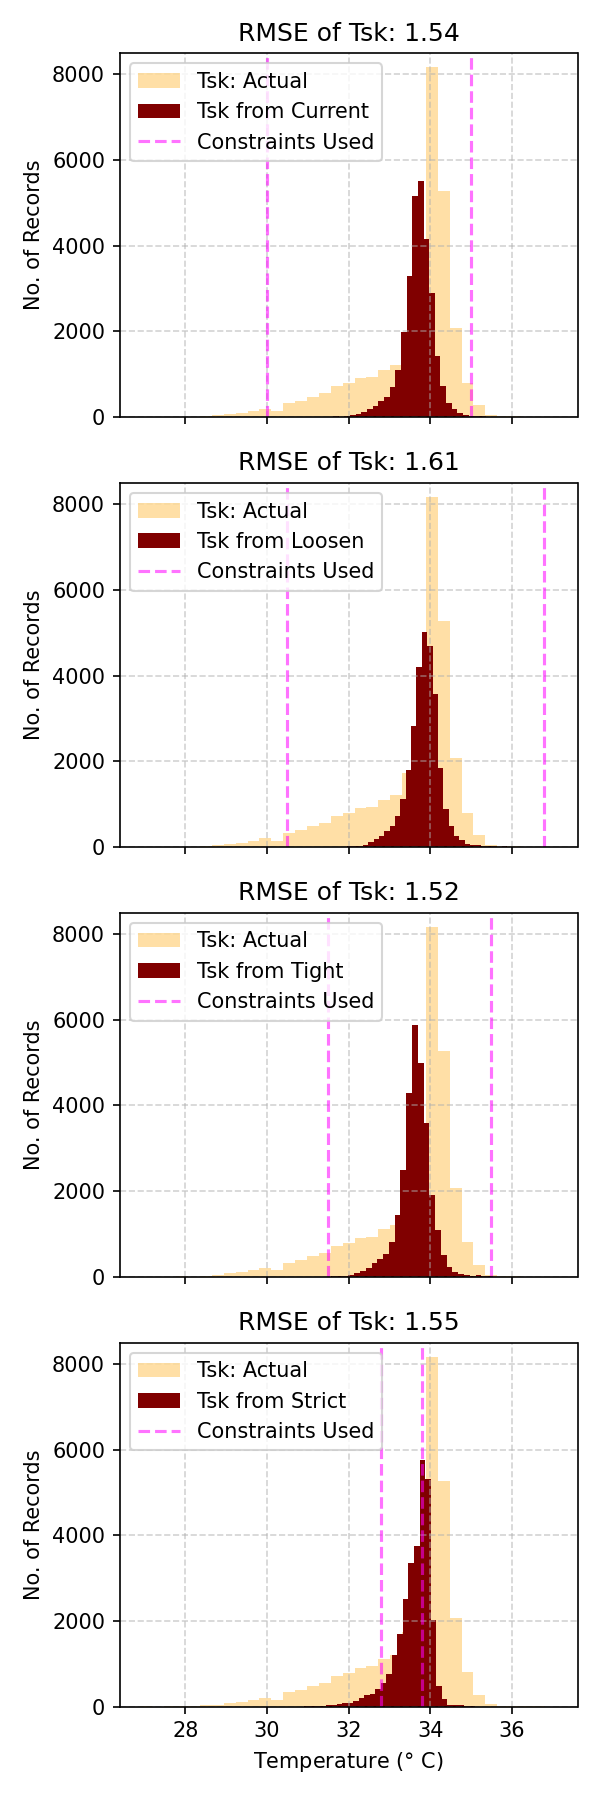
\includegraphics[width=0.49\linewidth]{figures/Tsk_dist.png}
    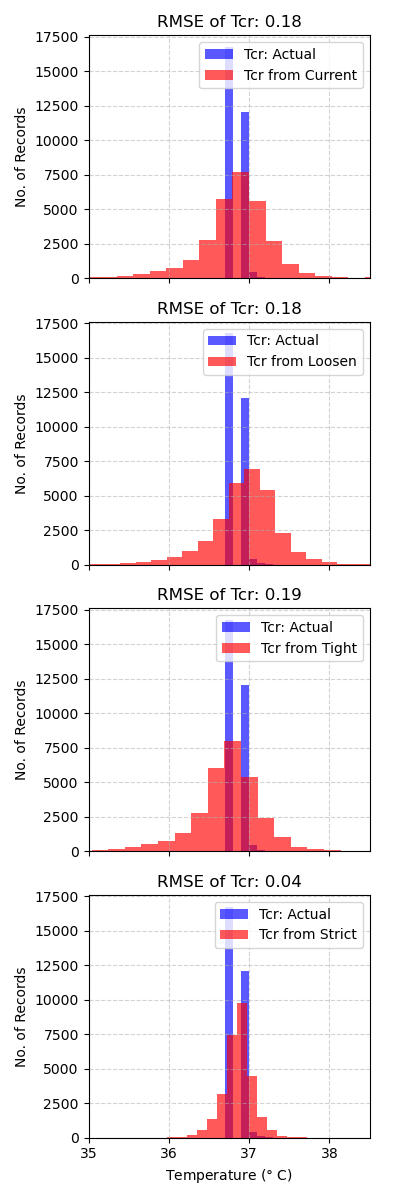
\includegraphics[width=0.49\linewidth]{figures/Tcr_dist.png}
    % \caption{Distribution of intermediate output between different variations of models}
    \label{fig:dist-cr-sk}
\end{figure}

\section*{Figure S2. Regression coefficients between $TSV$ and intermediate outputs}
\begin{figure}[H]
    \centering
    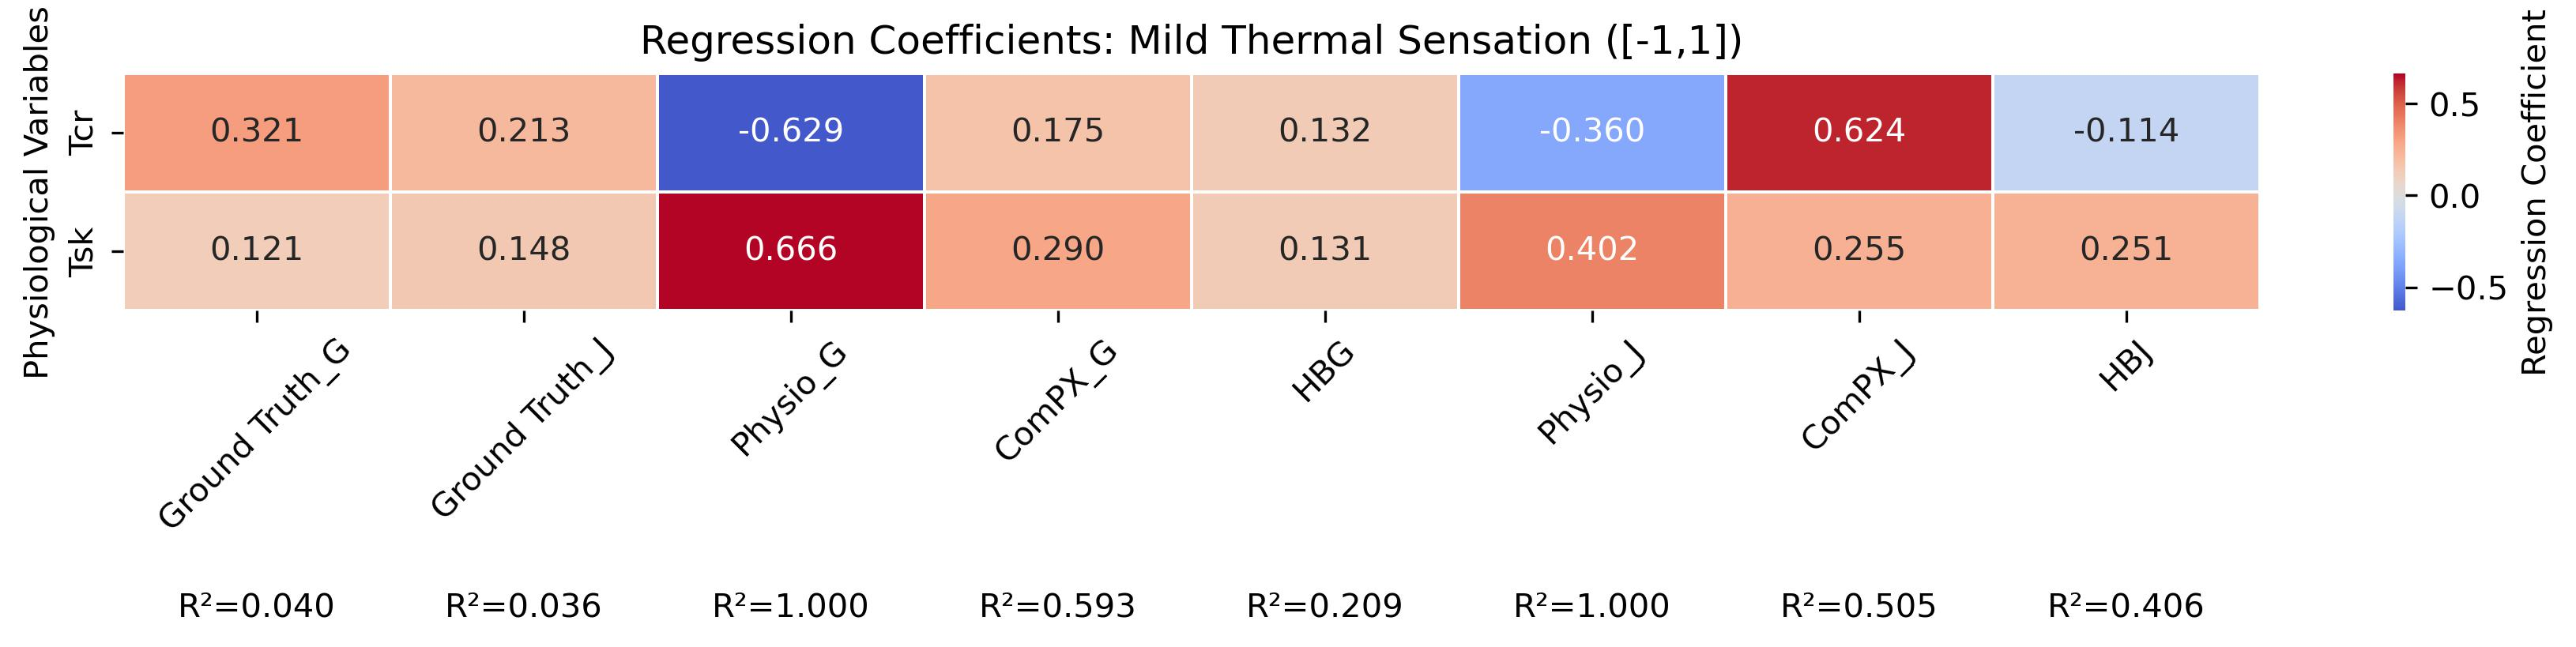
\includegraphics[width=\linewidth]{figures/regression_coef_Mild Thermal Sensation ([-1,1]).jpg}
    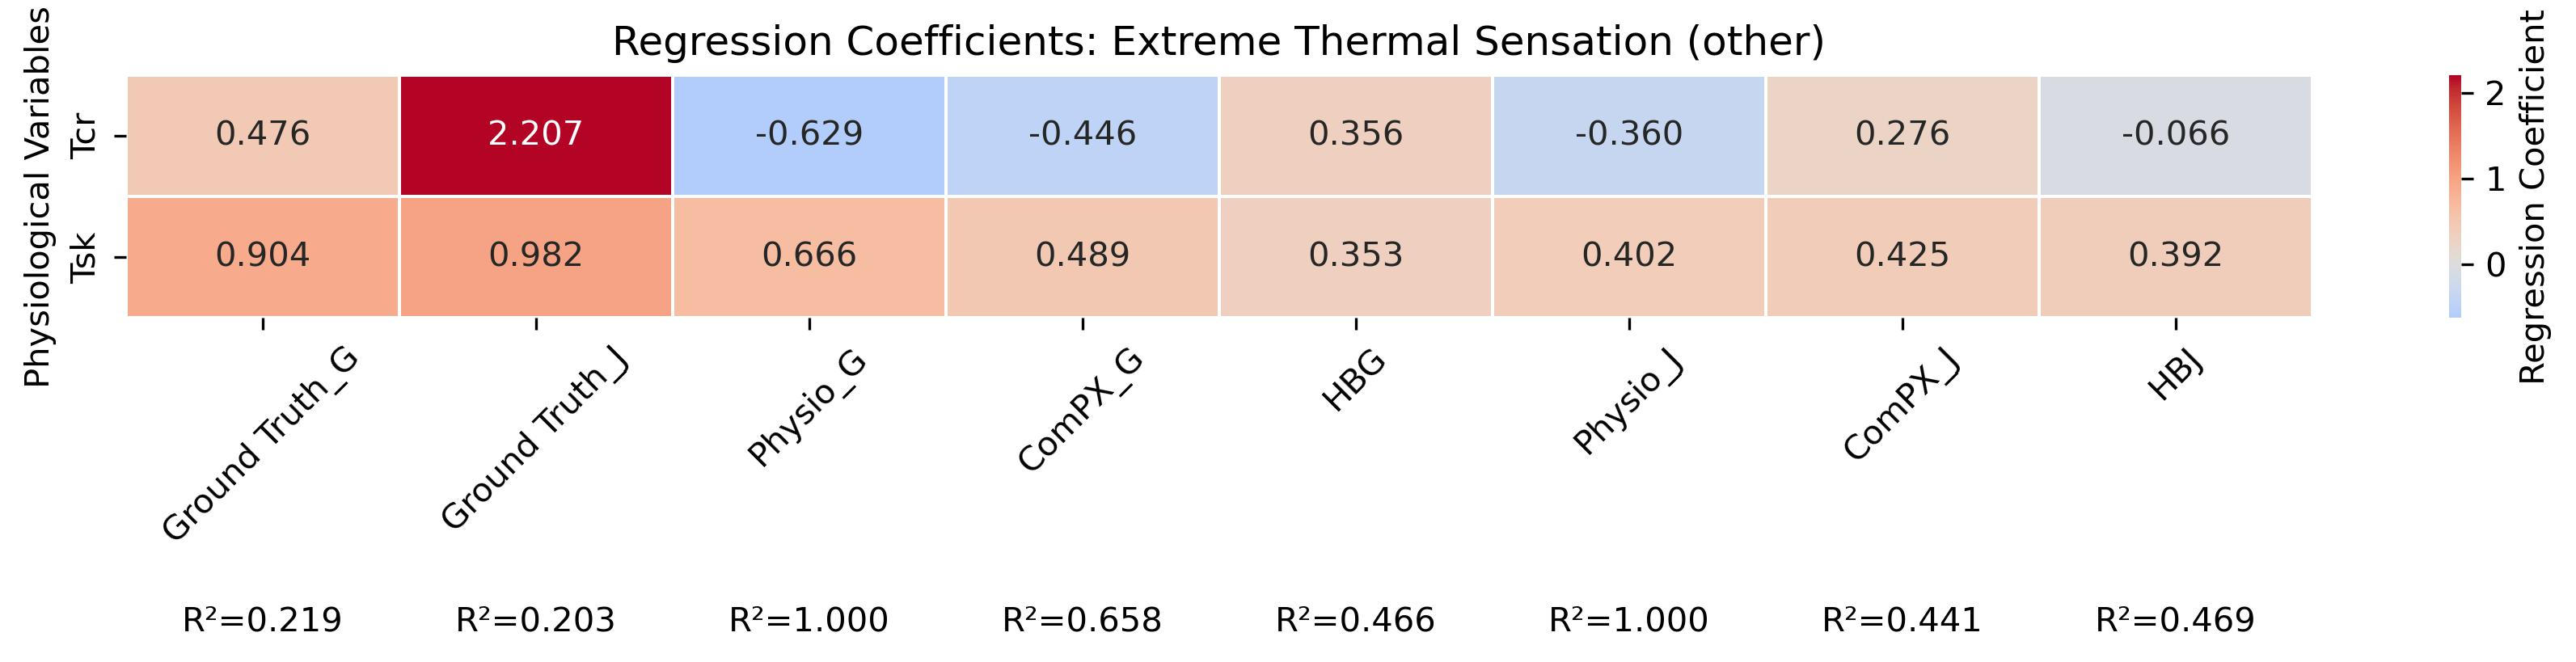
\includegraphics[width=\linewidth]{figures/regression_coef_Extreme Thermal Sensation (other).jpg}
    % \caption{Regression Coefficients under Mild (above) and Extreme (below) Thermal Sensation}
    \label{fig:regre-co}
\end{figure}

\end{document}

